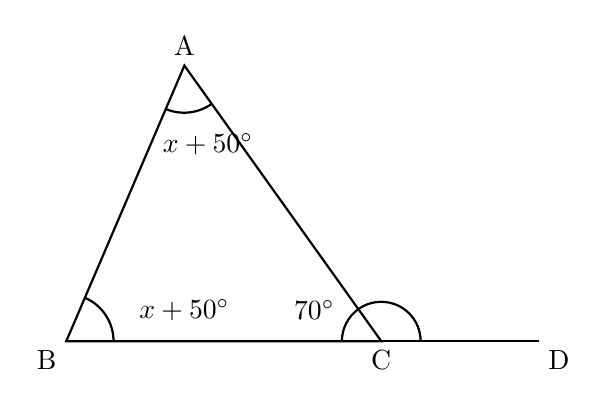
\begin{tikzpicture}[scale=1]

    % Define coordinates
    % Point A is shifted more to the left to match the visual proportions
    \coordinate (B) at (0, 0);
    \coordinate (C) at (4, 0);
    \coordinate (D) at (6, 0);
    \coordinate (A) at (1.5, 3.5);

    % Draw the main edges of the triangle ABC
    \draw[thick] (B) -- (A) -- (C) -- cycle;

    % Draw the extended line from C to D
    \draw[thick] (C) -- (D);

    % Draw the arc for interior angle B
    % Line BC is at 0 degrees. Line BA is at approx 66.8 degrees.
    \draw[thick] (0.6, 0) arc (0:66.8:0.6);
    % Add the angle label for B
    \node at (1.5, 0.4) {$x+50^{\circ}$};

    % Draw the arc for interior angle A
    % Line AB angle is approx 246.8 degrees. Line AC angle is approx 305.5 degrees.
    \draw[thick] (1.26, 2.95) arc (246.8:305.5:0.6);
    % Add the angle label for A
    \node at (1.8, 2.5) {$x+50^{\circ}$};

    % Draw the arc for interior angle C (left of C)
    % Line CB is at 180 degrees. Line CA is at approx 125.5 degrees.
    % The arc goes from 125.5 degrees to 180 degrees with radius 0.5
    \draw[thick] (3.71, 0.407) arc (125.5:180:0.5);
    % Add the angle label for interior angle C
    \node at (3.15, 0.4) {$70^{\circ}$};

    % Draw the arc for exterior angle ACD
    % Line CD is at 0 degrees. Line CA is at approx 125.5 degrees.
    % The arc goes from 0 degrees to 125.5 degrees
    \draw[thick] (4.5, 0) arc (0:125.5:0.5);

    % Add text labels to all vertices exactly as positioned in the image
    \node[above] at (A) {A};
    \node[below left] at (B) {B};
    \node[below] at (C) {C};
    \node[below right] at (D) {D};

\end{tikzpicture}